\documentclass[a4paper, upjsfrontpage, thesismargins, thesislinespacing]{rnthesis}
\usepackage[slovak]{babel}
\usepackage[T1]{fontenc}
\usepackage[utf8]{inputenc}
\usepackage{graphicx}
\usepackage{caption}
\usepackage{titlesec}
\usepackage{listings}

\titleformat{name=\chapter,numberless}
  {\normalfont\Large\bfseries}
  {}
  {0pt}
  {}

\captionsetup[table]{name=Tab.}
% disablespecwarning, usesections, {rnthesissvk}
\setcounter{secnumdepth}{4}

%%%%%%%%%%%%%%%%%%%%%%%%%%%%%%%%%%%%%%%%%%%%%%%%%%%%%%%%%%%%%%%%%%%%%%%%%%%%%%%%%%%%%%%%%%%%%%%%%%%%%%%%%%%%%%%%%%%%%%%%%%%%%%%

\title{Monitorovanie Informačných Systémov}
\author{Pavol Kozák}
\typprace{Bakalárska}
\pracovisko{Ústav informatiky}
\miesto{Košice}
\veduci{Doc. RNDr. Gabriel Semanišin PhD.}
\konzultant{RNDr. Erik Bruoth PhD.}
\rok{2015}

\podakovanie{Chcem sa poďakovať vedúcemu tejto práce Doc. RNDr. Gabrielovi Semanišinovi PhD., konzultantovi RNDr. Erikovi Bruothovi PhD. a Mgr. Slavomírovi Varchulovi za  cenné rady, odbornú pomoc a~konzultácie, ktoré mi poskytli pri vypracovaní tejto bakalárskej práce. \\ \\
Osobitné poďakovanie patrí mojej rodine a priateľom za podporu a pochopenie.}

\abstrakt{Hlavným cieľom našej bakalárskej práce je navrhnúť spôsob monitorovania informačného systému za účelom zbierania užitočných informácií ohľadom výkonu systému a používateľských preferenciách. Zaoberáme sa najmä otázkami aké informácie zbierať a akými nástrojmi ich zbierať. Existuje množstvo nástrojov z časti riešiacich našu problematiku. Zameriame sa na open-source nástroje. V práci si rozoberieme tie najpoužívanejšie, ich výhody a nevýhody a vybrané nástroje integrujeme do akademického informačného systému AiS2. Pomocou nich sa pokúsime zbierať a zobrazovať metriky, ktoré nám pomôžu identifikovať problémy a funkcie, ktoré je potreba vylepšiť.}

%%%%%%%%%%%%%%%%%%%%%%%%%%%%%%%%%%%%%%%%%%%%%%%%%%%%%%%%%%%%%%%%%%%%%%%%%%%%%%%%%%%%%%%%%%%%%%%%%%%%%%%%%%%%%%%%%%%%%%%%%%%%%%%

\begin{document}
\maketitle
\newpage

\setcounter{tocdepth}{2}
\tableofcontents

\newpage

%%%%%%%%%%%%%%%%%%%%%%%%%%%%%%%%%%%%%%%%%%%%%%%%%%%%%%%%%%%%%%%%%%%%%%%%%%%%%%%%%%%%%%%%%%%%%%%%%%%%%%%%%%%%%%%%%%%%%%%%%%%%%%%

\chapter*{Úvod}
\addcontentsline{toc}{chapter}{Úvod}

S informačnými systémami sa stretávame v dnešnej dobe čoraz častejšie. 
Mnohé systémy sa presúvajú z papierovej formy do elektronickej.
Môže to byť spôsobené mnohými výhodami tohto prechodu, ako napríklad jednoduchší prístup k informáciám, alebo len modernizáciou systému kvôli pokroku doby.

V tejto informačnej spoločnosti každý túži po informáciách.
S informačnými systémami sa stretávame na školách, na univerzitách, na pracoviskách, v zdravot\-níc\-tve a~v~rôznych iných oblastiach.

Vývojári informačných systémov sa snažia poskytnúť svojím zákazníkom informácie, ktoré hľadajú, kvôli ktorým navštívili ich informačný systém.
Aby vedeli, či ich systém funguje spoľahlivo, potrebujú ho nejakým spôsobom odmerať.

Na meranie systémov slúžia metriky.
Dávajú nám komplexnú informáciu o~systéme, o jeho nedostatkoch, o tom, čo vyžaduje zlepšenie, o rýchlosti a~spoľahli\-vos\-ti systému.
Pri zlepšovaní systému sú metriky veľmi užitočné.
Odhalia slabé miesta systému, ktoré by sme pri bežnom testovaní nespozorovali.

%%%%%%%%%%%%%%%%%%%%%%%%%%%%%%%%%%%%%%%%%%%%%%%%%%%%%%%%%%%%%%%%%%%%%%%%%%%%%%%%%%%%%%%%%%%%%%%%%%%%%%%%%%%%%%%%%%%%%%%%%%%%%%%

%\section{Základné pojmy}
\chapter{Základné pojmy}

%\subsection{Motivácia}
%\section{Motivácia}

%------------------------------------------------------------------------------------------------------------------------------

%\subsection{Informačný Systém}
\section{Informačný systém}

Informačný systém je zostavený z ľudí a počítačov, ktorí spracúvajú a interpretujú informácie.
Niekedy sa tento termín používa na označenie softvéru, ktorý využíva počítačovú databázu alebo len počítačového systému.
%\cite{website:wikipedia-informacnysystem}

V tejto práci sa budeme zameriavať na informačné systémy, ktoré sú vo forme webovej aplikácie.

%------------------------------------------------------------------------------------------------------------------------------

%\subsection{Webová Aplikácia}
\section{Webová aplikácia}

Webová aplikácia je aplikácia typu klient-server vytvorená pre prostredie internetu alebo intranetu.
V softvérovom inžinierstve je aplikácia poskytovaná užívateľom z~webového servera cez počítačovú sieť Internet, 
alebo jej vnútropodni\-kovú obdobu (intranet). 
Webové aplikácie sú populárne predovšetkým pre všade\-prítomnosť webového prehliadača ako klienta. 
Ten sa nazýva tenkým klientom, pretože sám o sebe logiku aplikácie nepozná.
Výhodou webových aplikácií je rovnaké užívateľské rozhranie kdekoľvek bez nutnosti inštalácie špeciálneho softvéru. 
Veľkou výhodou pre užívateľa ale aj pre prevádzkovateľa aplikácie je~jednoduchá aktualizácia. 
Tá sa vykonáva len na~jednom mieste - na serveri, na~ktorom webová aplikácia beží. Nevýhodou je nutnosť internetového pripojenia.
%\cite{website:wikipedia-webaplikacia}

%------------------------------------------------------------------------------------------------------------------------------

%\subsection{Metrika}
\section{Metrika}

%http://epodnikanie.euin.org/node/126
Slovo metrika je často používaný pojem v oblasti monitorovania systémov.
Metri\-ky v oblasti monitorovania sú spôsoby a nástroje merania, vyjadrujú stav určitého systému, 
napríklad jeho kvality, efektívnosti a nadobúdajú pri tom rôzne hodnoty. 
Pri riadení sa používajú indikátory aj pre definíciu a dosahovanie cieľov prípadne ich žiaducich hodnôt. 
Používajú sa tiež špecializované pojmy Performance indicator alebo Key performance indicator.
%\cite{website:epodnikanie}
Metriky nám pomáhajú ‘‘odmerať’’ systém a tým nám dávajú komplexnú informáciu o systéme a pomáhajú odhaliť jeho slabé miesta.
Vhodne zvolené metriky dokážu nasmerovať vývojárov správnym smerom a poukázať na možné problémy a tým v konečnom dôsledku pomôžu zlepšiť monitorovaný systém.

%\subsubsection{Rozdelenie Metrík}
\subsection{Rozdelenie metrík}

Medzi základné delenia metrík patrí delenie na kvalitatívne a kvantitatívne metriky.
Kvantitatívne metriky udávajú číselnú hodnotu, zatiaľ čo kvalitatívne metriky nečíselnú hodnotu.  
Kvantitatívne metriky sa ľahšie zobrazujú, interpretujú a sú zrozumiteľnejšie.
~\\
~\\
Metriky môžeme rozdeliť podľa druhu na:

\begin{itemize}
	\item výkonnostné metriky
	\item softvérové metriky
	\item aplikačné metriky
	\item systémové metriky
	\item používateľské metriky
\end{itemize}

V tejto práci nás budú zaujímať aplikačné, systémové a používateľské metriky.

%\subsubsection{Aká je Dobrá Metrika?}
\subsection{Aká je dobrá metrika?}

Aby metrika plnila svoj cieľ, teda podala správnu informáciu o systéme, mala by byť:
\begin{itemize}
	\item jednoduchá
	\item relevantná
	\item aktuálna
	\item okamžite ukončiteľná
\end{itemize}

Metrika by mala byť jednoduchá, aby bola ľahko interpretovateľná a pochopiteľná.
Relevantná metrika je taká, ktorá pomôže splniť cieľ, dosiahnuť to, na~čo~bola určená.
Neaktuálne metriky nám poskytnú možno už~nep\-ravdivé dáta a preto by metriky mali byť čo najaktuálnejšie. 
Len aktuálne dáta nám popíšu systém spoľahlivo.
Od metriky požadujeme, aby bola okamžite ukončiteľná, aby hneď po jej získaní bola pripravená na spracovanie a tak viedla k novým poznatkom.
%\cite{website:web-analytics.wikidot}

%\subsubsection{Typy Metrík}
\subsection{Typy metrík}

Medzi základné typy metrík patria údaje o počte (counting), údaje o čase (timing), iné číselné hodnoty (celočíselné alebo desatinné), alebo niekedy aj nečíselné hodnoty (gauges). 

Údajmi o počte môžeme získavať metriky ako napríklad počet požiadaviek, ktoré prišli na server za nejaký časový interval, počet volaní metódy v kóde, počet kliknutí na tlačidlo v informačnom systéme. Metriky tohto typu zbierame inkrementovaním počítadla v nástroji ako metrics alebo statsd v klientskej časti.

Často potrebujeme zmerať časový údaj ako napríklad čas pripojenia k databáze, čas obsluhy požiadavky alebo čas strávený vykonávaním určitého kusu kódu. Zmeraný čas zaznamenáme nástrojom na zbieranie metrík.

Niekedy je užitočné zbierať hodnotu, ktorá nezávisí od predchádzajúcich hodnôt napríklad počet objektov v rade, veľkosť dát odoslanej odpovede, alebo zaťaženie procesora. 
Tieto hodnoty môžu byť číselné alebo nečíselné. Tieto hodnoty pravidelne zbierame a odosielame na spracovanie a zobrazenie.

%------------------------------------------------------------------------------------------------------------------------------

%\subsection{Monitorovanie systému AiS2}
\section{Monitorovanie systému AiS2}

V našej bakalárskej práci chceme navrhnúť systém monitorovania akademického informačného systému AiS2.
Problémom je to, že vývojári systému AiS2 nie sú správcami systému.
Nemôžu preto získavať metriky ako napríklad zaťaženie serverov, voľná operačná pamäť, či iné systémové metriky, pretože tie sú skreslené virtualizáciou.
Tento problém sa týka aj cloudových riešení, ktorých v dnešnej dobe rýchlo pribúda.
Nemôžeme teda monitorovať priamo infraštruktúru aplikácie.
Aby vývojári zabezpečili hladký chod systému, musia sa spoľahnúť na aplikačné metriky.
Tie nám dajú informácie o aktuálnom stave aplikácie a o jej správaní.

Keďže systém AiS2 beží vo viacerých inštaláciách, 
	je potrebné monitorovať viacero inštalácií tohto systému samostatne, aj ako celok.
Chceme ich vedieť porovnať medzi sebou, 
	aby sme vedeli odlíšiť problémy v konkrétnej inštalácii a globálne problémy týkajúce sa systému samotného.
Na porovnanie inštalácií potrebujeme získané metriky mať na jednom mieste, na jednom serveri, čo môže výrazne skomplikovať zber metrík.
Potrebujeme zobrazovať agregované metriky zo všetkých inštalácií.
Bude jednoduchšie inštalácie porovnať a analyzovať nazbierané metriky.

Ďalším cieľom monitorovania systému AiS2 je optimalizácia interakcie systému s používateľom.
Chceme detekovať zle navrhnuté dialógy, ich neprehľadné umiestnenie v systéme, a analyzovať interakciu s používateľmi, napríklad aj dynamickým upravovaním používateľského rozhrania.

%------------------------------------------------------------------------------------------------------------------------------

%\subsection{Problémy}
\section{Problémy}

Hlavným cieľom monitorovania informačného systému je identifikovať problémy skôr ako používateľ.
Ak zbadá problém používateľ, už je neskoro.
Medzitým, ako nahlási problém vývojárom informačného systému, tento problém už mohlo zaznamenať množstvo ďalších používateľov.
Vývojári potom musia rýchlo problém identifikovať a opraviť, čo môže byť netriviálna záležitosť.
Ak by sme problém zaznamenali hneď ako nastane, mali by sme viac času na jeho riešenie.

Problém môže nastať, ak máme metrík veľa.
Monitorovanie systému nesmie systém výrazne zaťažiť, lebo by monitorovanie nebolo efektívne.

%------------------------------------------------------------------------------------------------------------------------------

%\subsection{Ilustračný Príklad}
\section{Ilustračný príklad}

Dobrým príkladom informačného systému je akademický informačný systém.
Monitorovanie takéhoto systému môže výrazne pomôcť k jeho vylepšeniu a~rozví\-janiu.

Ak by mal vývojár informáciu o prehliadačoch, ktorými sa používatelia pripojili do~systému, vedel by sa lepšie rozhodnúť, ktoré prehliadače má podporovať, aby pokryl čo najväčšiu skupinu používateľov.

Zaujímavou metrikou je aj rozlíšenie obrazoviek klientov, lebo s takouto informáciou sa dá lepšie rozvrhnúť používateľské rozhranie a zabezpečiť, aby klienti našli informácie, ktoré potrebujú rýchlejšie.
Ak by napríklad väčšina používateľov systému k nemu pristupovala s malou obrazovkou cez mobilný telefón, vývojár by investoval viac času a prostriedkov do prispôsobenia rozhrania pre mobilné telefóny.

Ďalšou zaujímavou metrikou je čas odpovede na požiadavku od klienta.
Ak zaznamenáme výrazne zvýšenie času odpovede vzhľadom na dlhodobý historický trend, vieme, že v systéme dochádza k problému a treba ho čo najskôr začať riešiť.

%------------------------------------------------------------------------------------------------------------------------------

%\subsection{Prehľad Súčasného Stavu}
 \section{Prehľad súčasného stavu}

V tomto čase je množstvo informačných systémov, ktoré sú neustále vylepšované a~zdokonaľované a~tak je potreba ich monitorovať, aby sa dali ešte viac zlepšiť a~prispôsobiť zákazníkom.
Každý systém je špecifický, a tak aj jeho monitorovanie je jedinečné.
Vývojári sa snažia upraviť monitorovanie ich systému a prispôsobiť ho tak, aby im poskytol čo najviac vedomostí o ich systéme.

Existuje niekoľko nástrojov, ktoré čiastočne ponúkajú riešenia našich problémov či už ide o zbieranie metrík alebo ich vizualizáciu.
Tieto nástroje sú však väčšinou zamerané na zbieranie systémových metrík a my potrebujeme zbierať hlavne aplikačné metriky.
Patria tu jak platené (Datadog, Stackdriver, Librato), tak aj open-source nástroje (Statsd, Metrics, Cacti, Graphite, Zabbix, Ganglia, Naggios).
My sa zaoberáme open-source nástrojmi.

%------------------------------------------------------------------------------------------------------------------------------

%\subsection{Ciele Práce}
\section{Ciele práce}

%\begin{enumerate}
%	\item Navrhnúť spôsob monitorovania informačného systému v reálnom čase za~úče\-lom zhromažďovania informácií o výkonne systému a používateľských pre\-ferenciách.
%	\item Navrhnúť dátovú štruktúru pre uložené metriky z jednotlivých inštalácií a~vytvoriť jednoduché štatistické prehľady nad zozbieranými údajmi v závis\-losti od~charakteru údajov.
%	\item Analyzovať možnosti využitia monitorovania pre účely optimalizácie interakcie s používateľom.
%\end{enumerate}

Hlavným cieľom našej bakalárskej práce je navrhnúť spôsob monitorovania informačného systému v reálnom čase za~úče\-lom zhromažďovania informácií o výkonne systému a používateľských pre\-ferenciách. 
Chceme tak navrhnúť systém monitorovania akademického informačného systému AiS2.

Ďalším cieľom je navrhnúť dátovú štruktúru pre uložené metriky z jednotlivých inštalácií a~vytvoriť jednoduché štatistické prehľady nad zozbieranými údajmi v závis\-losti od~charakteru údajov.
Potrebujeme určiť čo najvhodnejší spôsob ukladania metrík, ich agregácie z viacerých inštalácií na jedno miesto a vhodným spôsobom ich zobraziť.

Chceme tiež analyzovať možnosti využitia monitorovania pre účely optimalizácie interakcie s používateľom, teda zistiť, ako sa monitorovaním dá dosiahnúť skvalitnenie informačného systému pre jeho používateľov.

Keďže už existujú nástroje, ktoré čiastočne riešia naše problémy, naším cieľom bude aj porovnať tieto nástroje, popísať si ich výhody a nevýhody, a určiť nástroje, ktoré by boli najvhodnejšie pre monitorovanie informačného systému AiS2.

\newpage

%\section{Návrh Riešenia}

%\subsection{Úvod k zberu metrík}

%%%%%%%%%%%%%%%%%%%%%%%%%%%%%%%%%%%%%%%%%%%%%%%%%%%%%%%%%%%%%%%%%%%%%%%%%%%%%%%%%%%%%%%%%%%%%%%%%%%%%%%%%%%%%%%%%%%%%%%%%%%%%%%

%\section{Algoritmus monitorovania informačného systému}
\chapter{Algoritmus monitorovania informačného systému}

Ak chceme získať užitočné dáta o systéme aby sme ich mohli analyzovať, musíme ich najprv zozbierať.
Pred zbieraním metrík si treba najprv dobre premyslieť, čo chceme zbierať, 
aké metriky sú pre nás vhodné a aký cieľ chceme zberom metrík dosiahnuť.
Treba si dobre a jasne definovať metriky, aby sme z~nich mali čo najväčší osoh.

%\section{Algoritmus monitorovania informačného systému}

Monitorovanie informačného systému od prípravy na monitorovanie až po analýzu výsledkov monitorovania sa dá popísať nasledujúcim algoritmom:

\begin{enumerate}
	\item Určenie cieľov monitorovania informačného systému.
	\item Výber vhodných metrík.
	\item Výber nástrojov na monitorovanie a zobrazovanie metrík.
	\item Integrácia nástrojov a metrík do informačného systému.
	\item Zber metrík.
	\item Analýza získaných metrík.
	\item Vyvodenie dôsledkov monitorovania.
\end{enumerate}

\subsection*{Určenie cieľov monitorovania informačného systému}

Určenie cieľov monitorovania informačného systému je dôležité.
Musíme si dobre premyslieť, na čo chceme monitorovanie zamerať, čo chceme zlepšiť, čo potrebujeme odmerať.
Taktiež je dôležité premyslieť si, čo urobíme s výsledkom monitorovania a nakoľko bude výsledok merania relevantný a pravdivý.
To závisí aj od metrík, ktoré si zvolíme, od času a obdobia, v ktorom systém budeme monitorovať.
Treba si ujasniť problémy, ktoré chceme vyriešiť pomocou monitorovania.

\subsection*{Výber vhodných metrík}

Na to, aby sme monitorovaním dosiahli stanovené ciele, musíme si zvoliť vhodné metriky, 
	ktoré nám poskytnú odpovede na naše otázky.
Každý systém je odlišný a tak neexistuje univerzálny návod, aké metriky si zvoliť.

Treba sa zamyslieť nad tým, aké údaje by nám pomohli, keby sme ich mali k dispozícii.
Ak potrebujeme získať informácie o používateľoch a o ich správaní v systéme, pomohli by nám používateľské metriky.
Ak potrebujeme získavať údaje o stave aplikácie, potom je pre nás vhodné zbierať aplikačné metriky.
Keď chceme zistiť, aký je výkon systému a ako sa správa systém pri zaťažení a pod akou záťažou je v konkrétnych obdobiach, potom by sme sa mali zamerať na systémové metriky.

\subsection*{Výber nástrojov na monitorovanie a zobrazovanie metrík}

Ak už máme definované metriky, ktoré chceme zbierať, v ďalšej časti prípravy na monitorovanie si zvolíme vhodné nástroje na zber 	metrík a na ukladanie a zobrazovanie metrík.
Môžeme si zbieranie, ukladanie a zobrazovanie metrík navrhnúť a implementovať aj po svojom, ale keďže je monitorovanie informačných systémov rozšírené, existujú už špecializované nástroje, ktoré nám pomôžu s monitorovaním a zabezpečia nám kompatibilitu s ďalšími nástrojmi.

Nástrojov, ktoré máme k dispozícii, je niekoľko.
V tejto práci si rozoberieme open-source nástroje na zbieranie metrík Statsd a Metrics a nástroje na zobrazovanie metrík Graphite, Zabbix a Ganglia.
Všetky nástroje sú odlišné a majú svoje výhody a nevýhody, ktoré si podrobnejšie popíšeme.
Nástroje si vyberieme podľa funkcionality, náročnosti integrácie a podľa veľkosti informačného systému.

\subsection*{Integrácia nástrojov a metrík do informačného systému}

Po výbere nástrojov na monitorovanie nasleduje integrácia vybraných nástrojov a metrík do systému.
Zložitosť integrácie a konfigurácie závisí od nástrojov, ktoré sme si zvolili a od komplexnosti monitorovaného systému.
Metriky zbierame v podobe counterov, timerov a gauges, prípadne im podobným alebo inak pomenovaným alternatívnym spôsobom podľa vybraných nástrojov.

\subsection*{Zber metrík}

Ak máme nakonfigurované nástroje na zber metrík a funkčné prepojenie nástroja na zber metrík s nástrojom na ukladanie a zobrazovanie metrík, nasleduje fáza samotného zbierania metrík a monitorovania informačného systému.
V tejto fáze sledujeme metriky, ktoré nám nástroj na zobrazovanie metrík vykresľuje v prehľadných grafoch.
Niektoré zobrazovacie nástroje umožňujú aj agregáciu grafov pre jednotlivé metriky, to znamená, že súvisiace metriky si zobrazíme v jednom spoločnom grafe. 

Niektoré nástroje, alebo ich jednoduché prepojenie s ďalším nástrojom ponúkajú možnosť notifikácie administrátora o udalostiach, ktoré nastali v systéme.
Môžeme tak byť notifikovaný napríklad o priveľkej záťaži na systém, o nedostatku voľnej operačnej pamäti alebo o pridlhom čase čakania klienta na odpoveď zo servera.
To nám pomôže identifikovať aktuálne nastávajúci problém, ktorý je potrebné čo najskôr vyriešiť.
Takisto nám to pomôže odhaliť problém skôr, ako ho odhalý používateľ nášho systému.

\subsection*{Analýza získaných metrík}

Ak už zbierame metriky dlhšiu dobu, máme dostatok údajov na ich analýzu a ďalšie spracovanie.
Môžeme analyzovať, ako sa systém správa v určitých obdobiach, ako sa správajú používatelia v systéme a ako sa správa systém, keď je pod záťažou. To nám pomôže pripraviť sa na ďalšiu záťaž, alebo zistíme, že potrebujeme zbierať ďalšie metriky, na ktoré sme na začiatku nemysleli, alebo sa nám zdali irelevantné.

\subsection*{Vyvodenie dôsledkov monitorovania}

V ďalšej fáze vyvodíme dôsledky monitorovania.
Zamyslíme sa, či nám monitorovanie pomohlo splniť ciele, ktoré sme si na začiatky stanovili a ako nám to pomohlo zlepšiť systém.
Porozmýšľame, čo nám ešte treba zlepšiť, aké závery nám plynú z monitorovania a určíme ďalšie kroky k ešte lepšiemu monitorovaniu.

Monitorovanie informačného systému je dlhodobý proces, a počas monitorovania sa môže meniť a upravovať s meniacím sa systémom a už získanými poznatkami z monitorovania.
Môžeme pridávať nové metriky aj s novou funkcionalitou alebo tie nepodstatné metriky zmazať.
V tejto fáze upravíme systém podľa výsledkov, ktoré sme získali monitorovaním.
Napríklad ak sme zistili, že náš systém potrebuje optimalizáciu dopytov do databázy, optimalizujeme ich a sledujeme, aký to ma dopad na systém a na rýchlosť odpovede na požiadavky od klientov.

Na obrázku 2.1 môžete vidieť životný cyklus monitorovania informačného systému.

\begin{figure}
\begin{center}
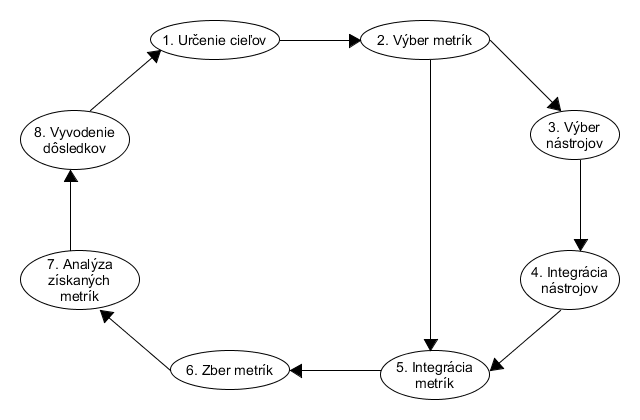
\includegraphics[scale=0.7]{ais_algorithm.png}
\caption{Životný cyklus monitorovania informačného systému}
\end{center}
\end{figure}

\newpage

%%%%%%%%%%%%%%%%%%%%%%%%%%%%%%%%%%%%%%%%%%%%%%%%%%%%%%%%%%%%%%%%%%%%%%%%%%%%%%%%%%%%%%%%%%%%%%%%%%%%%%%%%%%%%%%%%%%%%%%%%%%%%%%

%\section{Typy monitorovania}
\chapter{Typy monitorovania}

%------------------------------------------------------------------------------------------------------------------------------

%\subsection{Monitorovanie systému v reálnom čase}
\section{Monitorovanie systému v reálnom čase}

Monitorovanie systému v reálnom čase nám pomôže detekovať problém skôr, ako ho zbadá používateľ.
Prehľadné grafy zobrazujúce nazbierané metriky nám ukážu dôležité informácie o stave systému.
Niektoré nástroje nás dokonca upozornia, ak v systéme nastane problém.
Po vyriešení problému zas z grafov vyčítame, či sme detekovaný problém vyriešili a ako dobre sme ho vyriešili.

%------------------------------------------------------------------------------------------------------------------------------

%\subsection{Dlhodobé monitorovanie systému}
\section{Dlhodobé monitorovanie systému}

Krátkodobé merania systému nám podajú užitočnú informáciu o aktuálnom stave systému a o jeho používateľoch.
Nás však zaujímajú aj dlhodobé merania.
Tie nám povedia, kedy v priebehu roka je systém najviac zaťažený, kedy najmenej, a aké funkcionality používatelia využívajú v konkrétnych obdobiach.
To sa nám pomôže pripraviť na najväčšiu záťaž.

Po vylepšení niektorej funkcionality v systéme vieme porovnať nové hodnoty metrík s historickými hodnotami metrík pre danú funkcionalitu.
Dozvieme sa tak, či sme funkcionalitu naopak nezhoršili a či bude schopná vydržať záťaž.

%------------------------------------------------------------------------------------------------------------------------------

%\subsection{Monitorovanie systému za účelom hĺbkovej analýzy}
\section{Monitorovanie systému za účelom hĺbkovej analýzy}

Dlhodobými meraniami vieme zaznamenávať vzory správania používateľov v našom informačnom systéme.
Takýmto vzorom môže byť v akademickom informačnom systéme napríklad:

\begin{itemize}
	\item Používatelia si najčastejšie po prihlásení do aplikácie prečítajú nové správy.
	\item Po prečítaní správ sa odhlásia alebo:
	\begin{itemize}
		\item Ak je začiatok semestra, pozrú si rozvrh hodín.
		\item Ak je stred semestra, pozrú sa na priebežné hodnotenie.
		\item Ak je koniec semestra, prihlásia sa na skúšku.
	\end{itemize}
\end{itemize}

Ak získame takéto vzory, môžeme napríklad dynamicky meniť používateľské rozhranie počas priebehu semestra a sprístupniť tak najčastejšie hľadané informácie podľa vzorov na viditeľnejšie miesta v našom systéme.

Dlhodobými meraniami systému vieme získať aj ďalšie zaujímavé informácie.
Nad množstvom vyzbieraných metrík sa dá robiť hĺbková analýza v podobe dolovania dát.
No na hĺbkovú analýzu budeme potrebovať väčšinou odlišné dáta od tých, ktoré pre nás majú zmysel pri monitorovaní v reálnom čase.
Budú nás zaujímať iné metriky a aj ciele takejto analýzy budeme mať odlišné.

\newpage

%%%%%%%%%%%%%%%%%%%%%%%%%%%%%%%%%%%%%%%%%%%%%%%%%%%%%%%%%%%%%%%%%%%%%%%%%%%%%%%%%%%%%%%%%%%%%%%%%%%%%%%%%%%%%%%%%%%%%%%%%%%%%%%

%\section{Nástroje na Zber Metrík}
\chapter{Nástroje na zber metrík}

Ak už máme jasne definované metriky, môžeme ich začať zbierať.
Zber metrík je~často riešený problém, v zbere metrík nám môžu pomôcť rôzne nástroje.
Medzi naj\-populár\-nejšie open-source nástroje na zber metrík patria Metrics a Statsd.
Sú to nástroje určené na odosielanie nameraných metrík do nástrojov na uloženie a zobrazenie metrík v podobe grafov.

Integrácia oboch nástrojov si však vyžaduje určité zmeny v kóde systému.
Každý systém je jedinečný a teda aj jeho monitorovanie je odlišné.
To si však žiada odlišné metriky a tie sa zbierajú na odlišných miestach v kóde systému.

% rovnake nastroje, len ine riesenie zbieranie - "definovanie", cache, 
Oba nástroje sú funkcionalitou podobné, no odlišné z hľadiska integrácie a architektúry.
Riešia ten istý problém - definujú metriky v kóde systému a fungujú ako cache pre metriky, a po nastavenom časovom intervale ich posielajú ďalším nástrojom.
Naším čiastočným cieľom je porovnať ich.
V nasledujúcich odstavcoch si popíšeme ich výhody a nevýhody.

%------------------------------------------------------------------------------------------------------------------------------

%\subsection{Nástroj Metrics}
\section{Nástroj Metrics}

Metrics je open-source java knižnica na zber metrík.
Získané metriky posiela do nástrojov na zobrazovanie metrík ako napríklad Graphite alebo Ganglia, alebo ukladá do databázy prostredníctvom logovacích nástrojov.

Keďže Metrics je java knižnica, integrácia nástroja do java webovej aplikácie je~záležitosť pridania niekoľkých závislostí.
Následne definujeme registre, v ktorých budú metriky uložené.
Ďalej je potrebné nastaviť reportovanie do ďalších nástrojov.
Potom na vhodných miestach v aplikácii získame metriky pomocou counterov, timerov a gauges, ktoré chceme zbierať.
Nástroj Metrics nám pomôže dostať namerané metriky do~ďalších nástrojov.

Asi najväčšou konkurenciou k Metrics je nástroj Statsd.

%------------------------------------------------------------------------------------------------------------------------------

%\subsection{Nástroj Statsd}
\section{Nástroj Statsd}

Open-source nástroj Statsd je určený na zber metrík a následné preposlanie do nástrojov na spracovanie a zobrazenie.
Má kientov pre množstvo programovacích jazykov ako napríklad node.js, java, python, ruby, perl, php, c, cpp, .net, či dokonca plugin pre wordpress. 

% cez siet
Statsd klient na rozdiel od Metrics posiela získane metriky cez sieťovú komunikáciu na otvorený UDP port na oddelený Statsd server, ktorý ich prijíma, akumuluje a odosiela do ďalších nástrojov. 
Slúži ako rýchla cache pre metriky. 
Umožňuje posielať dáta do nástrojov ako napríklad Graphite, Ganglia, Librato, Zabbix, či Mongo, Mysql, Datadog a mnoho ďalších.

Architektúra tohto nástroja je trochu zložitejšia.

%------------------------------------------------------------------------------------------------------------------------------

%\subsection{Metrics vs Statsd}
\section{Metrics vs Statsd}

Obe nástroje slúžia na zbieranie metrík, majú však rozdielnú architektúru. 
Ponúkajú rôzne možnosti integrácie s ďalšími nástrojmi. 
Kvôli prehľadnosti sú základné rozdiely popísané v tabuľke 4.1.
Údaje v tabuľke 4.1 sú aktuálne vzhľadom k času písania bakalárskej práce.

\begin{table}
	\caption{Porovnanie nástrojov Metrics a Statsd}
	\centering
	\begin{tabular}{| p{3.7cm} | p{4.5cm} | p{4.7cm} |}
		\hline\noalign{\smallskip}
		Atribút porovnania & Metrics & Statsd \\
		\noalign{\smallskip}
		\hline
		Architektúra & Server totožný s klientom & Server a klient oddelený \\ \hline

		Integrácia s ďalšími nástrojmi & Ganglia, Graphite, Librato, Spring, Sematext, Wicket, Guice, Scala, Clojure, Cassandra, 	Elasticsearch, Statsd, Datadog, Influxdb, Cdi, Aspectj, Apache Camel & Amqp, Ganglia, Librato, Socket.io, Statsd, Mongo, Mysql, Datadog, Monitis, Instrumental, Hosted graphite, Zabbix, Opentsdb, Influxdb, Stackdiver, Couchdb \\ \hline

		Implementácia Servera & Iba Java & Node.js, Python, Ruby, C, Go, Clojure, 	Perl \\ \hline

		Implementácia Klienta & Klient totožný so serverom & Node.js, Java, Python, Ruby, Perl, Php, Clojure, C, Cpp, .Net, Go, 	Apache, Io, Varnish, PowerShell, JavaScript, Cocoa, ActionScript, Wordpress \\ \hline

		Licencia & Apache 2 & MIT \\ \hline

		Zložitosť integrácie do java webovej aplikácie & Import knižnice, definovanie metrík, nastavenie reportovania & Inštalácia Node.js, Statsd servera, import Statsd klientskej knižnice, definovanie metrík, inštalácia reportovacích backendov, konfigurácia Statsd servera \\ \hline

		Počet prispievateľov & 127 & 154 \\ \hline

		Počet verzií & 51 & 11 \\ \hline

		Prvý príspevok do repozitára & 27.4.2011 & 30.12.2010 \\ \hline
		
		Počet príspevkov do repozitára & 1958 & 823 \\ \hline

		%Dokumentácia & Dostatočná & Dostatočná \\ \hline
	\end{tabular}
\end{table}

\newpage

%%%%%%%%%%%%%%%%%%%%%%%%%%%%%%%%%%%%%%%%%%%%%%%%%%%%%%%%%%%%%%%%%%%%%%%%%%%%%%%%%%%%%%%%%%%%%%%%%%%%%%%%%%%%%%%%%%%%%%%%%%%%%%%

%\section{Nástroje na Ukladanie a Zobrazenie Metrík}
\chapter{Nástroje na ukladanie a zobrazenie metrík}

Nástroje na zbieranie metrík majú často za úlohu agregovať metriky a preposielať ich do ďalších nástrojov.
Existujú rôzne nástroje na~ukladanie a zobrazenie metrík.
Niektoré z nich sú komerčné, iné open-source.
Medzi často používané open-source nástroje patria nástroje Graphite, Zabbix a Ganglia.
Tieto nástroje vedia prijať dáta z iných nástrojov, uložiť ich v databáze a~vhodným spôsobom ich zobraziť, aby sa dali ľahšie interpretovať.

Rôzne nástroje na zbieranie metrík majú rôznu architektúru a ponúkajú rozličnú funkcionalitu.
Záleží od veľkosti a komplexnosti systému a aj od požadovanej funkcionality, ktorý nástroj si vyberieme.

Metriky sa najčastejšie zobrazujú v podobe histogramov alebo čiarových diagramov cez používateľské rozhranie vo forme webovej aplikácie.

%------------------------------------------------------------------------------------------------------------------------------

%\subsection{Nástroj Graphite}
\section{Nástroj Graphite}

Nástroj Graphite je veľmi obľúbeným nástrojom v oblasti zobrazovania metrík.
Nástroje ako napríklad Statsd alebo Metrics pošlú získané metriky do Graphitu a ten ich uloží pomocou integrovaného nástroja Carbon do Whisper databázy. 
Whisper databáza je veľmi podobná RRD (round robin database) databáze, ale je prispôsobená a~napísaná v pythone.
Kód graphitu je napísaný v programovacom jazyku python.
Metriky stačí poslať do nástroja Graphite a on ich sám zaradí do stromu metrík podľa prefixu.
Po inštalácii sa nevyžaduje žiadna dodatočná konfigurácia.

Na obrázku 5.2 môžete vidieť používaťeľské rozhranie nástroja Graphite a čiarový diagram pre metriku zaťaženie procesora.

\begin{figure}
\begin{center}
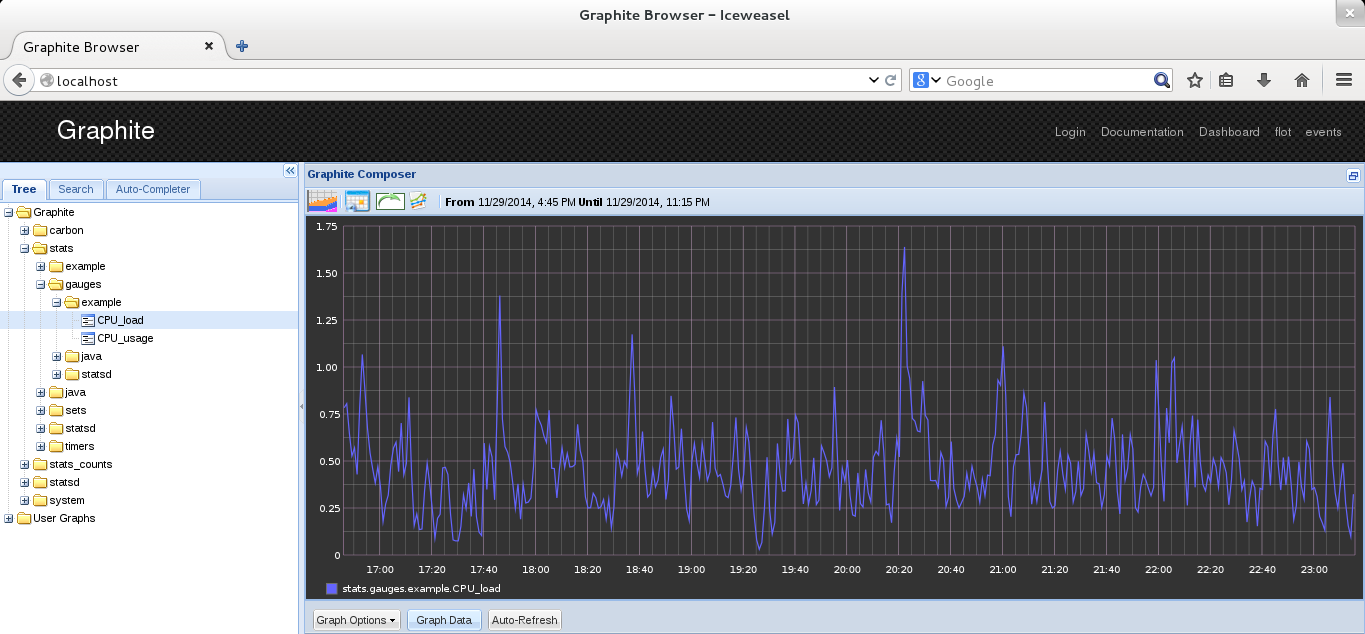
\includegraphics[scale=0.41]{graphite1.png}
\caption{Používateľské rozhranie nástroja Graphite}
\end{center}
\end{figure}

Nástroj Graphite je jednoduchý open-source nástroj určený na ukladanie a zobrazovanie metrík v podobe grafov.
Na vykresľovanie grafov využíva python knižnicu PyCairo.
V praxi sa používa pri jednoduchých projektoch, ak nám postačuje získané metriky zobrazovať.
Pri monitorovaní komplexnejších systémov sa používajú zložitejšie nástroje ako napríklad Zabbix alebo Ganglia.

%\subsubsection{Výhody nástroja Graphite}
\subsection{Výhody nástroja Graphite}

Graphite je jednoduchý nástroj určený pre monitorovanie malých jednoduchších systémov.
Hlavnou výhodou je, že po inštalácii nástroja sa nevyžaduje žiadna konfigurácia metrík.
Ďalšou výhodou je jednoduché zobrazenie viacerých metrík v jednom grafe.
Graphite je zameraný na monitorovanie systémov v reálnom čase.

%\subsection{Nevýhody nástroja Graphite}
\subsection{Nevýhody nástroja Graphite}

Nástroj Graphite je zameraný len na vykresľovanie metrík a neponúka žiadnú dodatočnú funkcionalitu.
Jeho nevýhodou je, že má komplikovanú inštaláciu.
Počas jeho inštalácie treba nainštalovať a nakonfigurovať všetky potrebné moduly, čiže Carbon, Whisper, Graphite web, Pycairo a Apache.
% dopisat komplikacie

%------------------------------------------------------------------------------------------------------------------------------

%\subsection{Nástroj Zabbix}
\section{Nástroj Zabbix}

Ďalším používaným nástrojom je Zabbix.
Jeho kód je napísaný v jazyku C a~používateľské rozhranie v podobe webovej aplikácie je napísaný v jazyku PHP.
Na ukladanie metrík používa Mysql databázu.
Na obrázku 5.3 môžete vidieť graf operačných systémov a prehliadačov používateľov systému AiS2 v Zabbixe.

% obrazok biely
\begin{figure}
	\begin{center}
		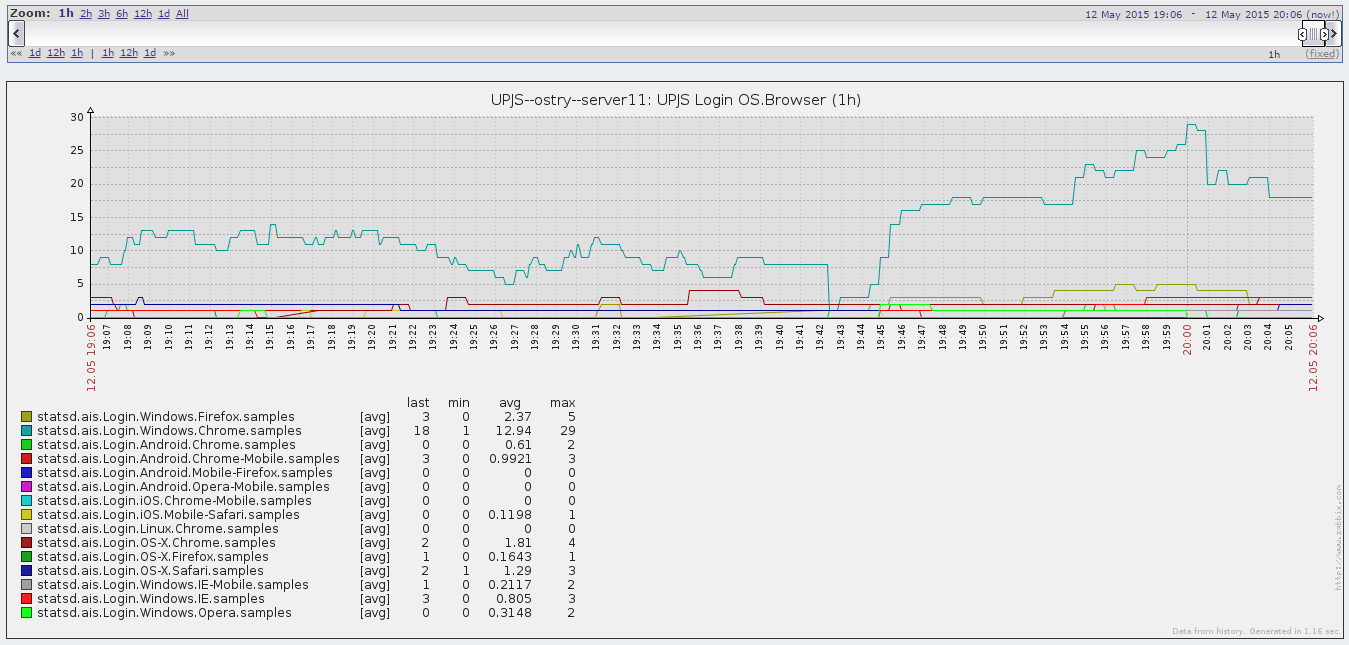
\includegraphics[scale=0.41]{zabbix1.png}
	\end{center}
	\caption{Graf prehliadačov používateľov systému AiS2 v Zabbixe}
\end{figure}

Zabbix je komplexný nástroj určený aj pre väčšie systémy.
Okrem vizualizácie dokáže zbierať vlastné metriky, pomáha detekovať problém a vie o ňom notifikovať administrátorov.
Je to omnoho mohutnejší nástroj ako Graphite.

K informačnému systému patrí aj hardvér, na ktorom systém beží.
Informácie o hardvéri a rôzne iné systémové metriky môžeme zbierať pomocou modulu Zabbix agent.
Zabbix agent pravidelne posiela získané udaje zo stroja, kde je nasadený na Zabbix server.
Môžeme tak jednoducho monitorovať napríklad výkon systému, sieťové zariadenia, virtuálne stroje, databázy, Java virtual machine alebo Java aplikačné servery.

Zabbix tiež umožňuje na zber dát použiť SNMP a IPMI agentov alebo Zabbix sender nástroj, ktorým do Zabbixu vieme poslať ľubovoľné metriky z nástrojov na zbieranie metrík.

Zabbix môže slúžiť aj na detekciu problémov so systémom.
Detekcia problémov v Zabbixe funguje pomocou definovania triggerov, ktoré odhalia, že niečo nefunguje.
Môže to byť napríklad výpadok stroja, málo voľného miesta na disku monitorovaného zariadenia alebo veľa pripojených používateľov.
V triggery sa nastavý prah, ktorým určíme maximálnu akceptovateľnú hodnotu metriky.

Ak sa táto hodnota prekročí, Zabbix nás o tom môže notifikovať alebo vykoná nastavenú akciu.
Môže nás notifikovať prostredníctvom e-mailu, SMS správy alebo správy cez Jabber.
Môžeme si tiež nastaviť, aké dáta sa nám v notifikácii zobrazia.
Okrem notifikačnej správy Zabbix vie po detekcii problému vykonať napríklad shell príkaz cez~ssh.

%\subsubsection{Výhody nástroja Zabbix}
\subsection{Výhody nástroja Zabbix}

Veľkou výhodou nástroja Zabbix je to, že na ukladanie metrík používa Mysql databázu.
Dáta tak máme uložené v relačnej databáze a vieme sa na ne jednoducho dopytovať.
To má potenciál na zber dlhodobých metrík za účelom hĺbkovej analýzy a dolovanie dát z týchto údajov.
% potencial na riesenie 


%\subsubsection{Neýhody nástroja Zabbix}
\subsection{Neýhody nástroja Zabbix}

Hlavná nevýhoda Zabbixu je to, že každá metrika, ktorú chceme monitorovať musí byť dopredu nakonfigurovaná.
Ak máme metrík veľa, úvodná konfigurácia je pracná.
Síce sa v Zabbixe dajú použiť šablóny, ktoré trochu zjednodušia konfiguráciu ale stále musíme všetky metriky nakonfigurovať ručne.
V systéme AiS2 sme tieto šablóny použili na definovanie rovnakých metrík pre rôzne servery.
Pri každej novej funkcionalite informačného systému s predpokladom, že ju chceme monitorovať, je potrebné nakonfigurovať nové metriky aj v Zabbixe.
% aj ked existuju templates pouzitie v AiSe

%------------------------------------------------------------------------------------------------------------------------------

%\subsection{Nástroj Ganglia}
\section{Nástroj Ganglia}

Dalším obľúbeným nástrojom je Ganglia.
Ganglia je open-source nástroj zameraný na~distribuované monitorovanie celých clustrov či gridov.
Je naozaj rozšírený, používajú ho napríklad známe spoločnosti ako Twitter, flickr, National Aeronautics and Space Administration (NASA), Wikipedia, CERN, Cisco, HP, Microsoft, Dell, nVidia, U.S. Air Force.

Metriky do Ganglie môžeme poslať pomocou Gmond modulov, Gmetric modulu alebo inými nástrojmi, ako napríklad statsd.
Ak posielame metriky do Ganglie, nemusíme ich mať dopredu nakonfiguroavné.
Gmetad vytvorí nový RRD súbor pre každú novú metriku, čo značne uľahčí konfiguráciu, ak metrík máme veľa.
Webové používaťeľské rozhranie potom zobrazí základný graf pre každú metriku.

Ganglia na posielanie metrík na centrálny server používa dvoch démonov a to Ganglia Monitoring Daemon (gmond) a Ganglia Meta Daemon (gmetad).
Gmond môže posielať alebo prijímať metriky, ktoré si drží v pamäti.
Gmetad v rámci gridu ťahá dáta z jedného gmond démona z každého clustra.
Gmond moduly so sebou komunikujú cez UDP protokol a do gmetad posielajú dáta v štruktúre XML cez TCP protokol.
Gmetad si medzi sebou posielajú metriky cez TCP vo forme XML.
Gmond medzi sebou kominikujú buď prostredníctvom unicastu alebo multicastu.

Ak použijeme unicast, komunikácia zo všetkých gmondov smeruje do jedného centrálneho gmond modulu v rámci clustera.
Gmetad potom zbiera dáta zo všetkých centrálnych gmond modulov.
Táto konfigurácia je výhodná, ak máme veľmi veľa uzlov (1000).
Architektúra s použitím unicastu je popísaná na obrázku 5.4.

Ak máme menší počet uzlov v gride, viac sa nám oplatí použiť multicast.
Po pridaní nových uzlov do clustra nie je potrebná dodatočná konfigurácia.
Architektúra s použitím multicastu je popísaná na obrázku 5.5.

\begin{figure}
	\begin{center}
		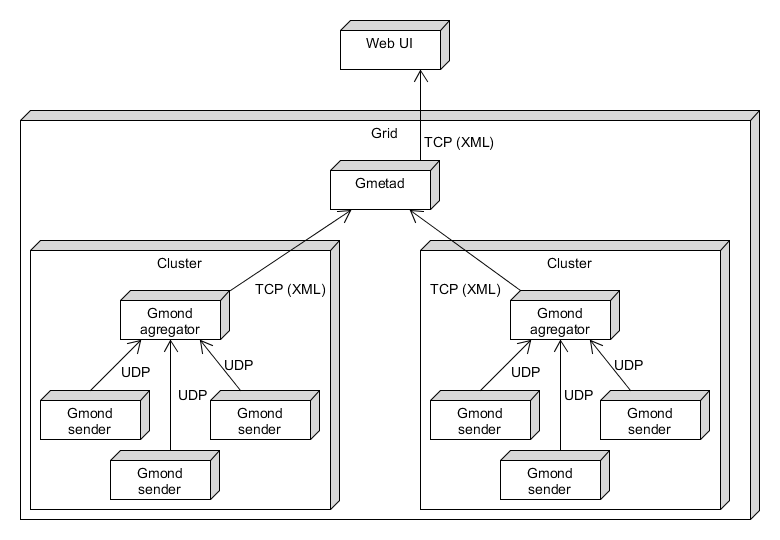
\includegraphics[scale=0.55]{ganglia-architecture.png}
	\end{center}
	\caption{Architektúra Ganglie s použitím unicastu}
\end{figure}

\begin{figure}
	\begin{center}
		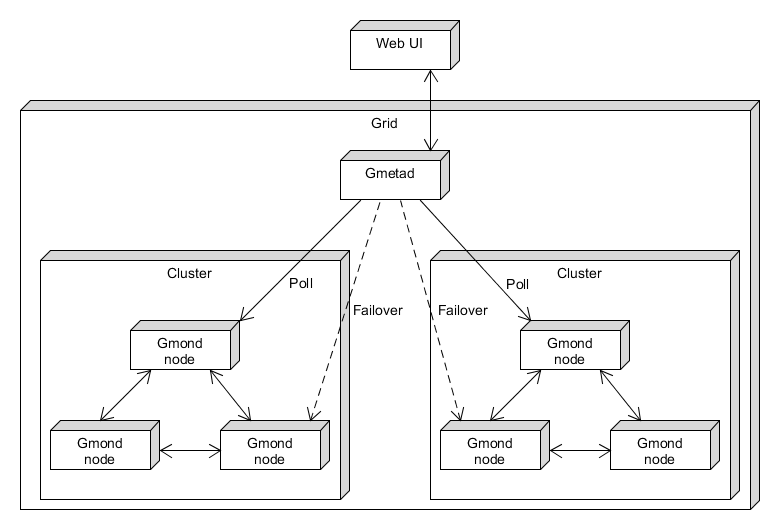
\includegraphics[scale=0.55]{ganglia-architecture-multicast.png}
	\end{center}
	\caption{Architektúra Ganglie s použitím multicastu}
\end{figure}

% pridat multicast obrazok

Ganglia priamo nepodporuje detekciu problémov v systéme.
Umožňuje však prepojenie s nástrojom Naggios, ktorý je na to určený.
Na obrázku 5.6 môžete vidieť používaťeľské rozhranie nástroja Ganglia.

\begin{figure}
	\begin{center}
		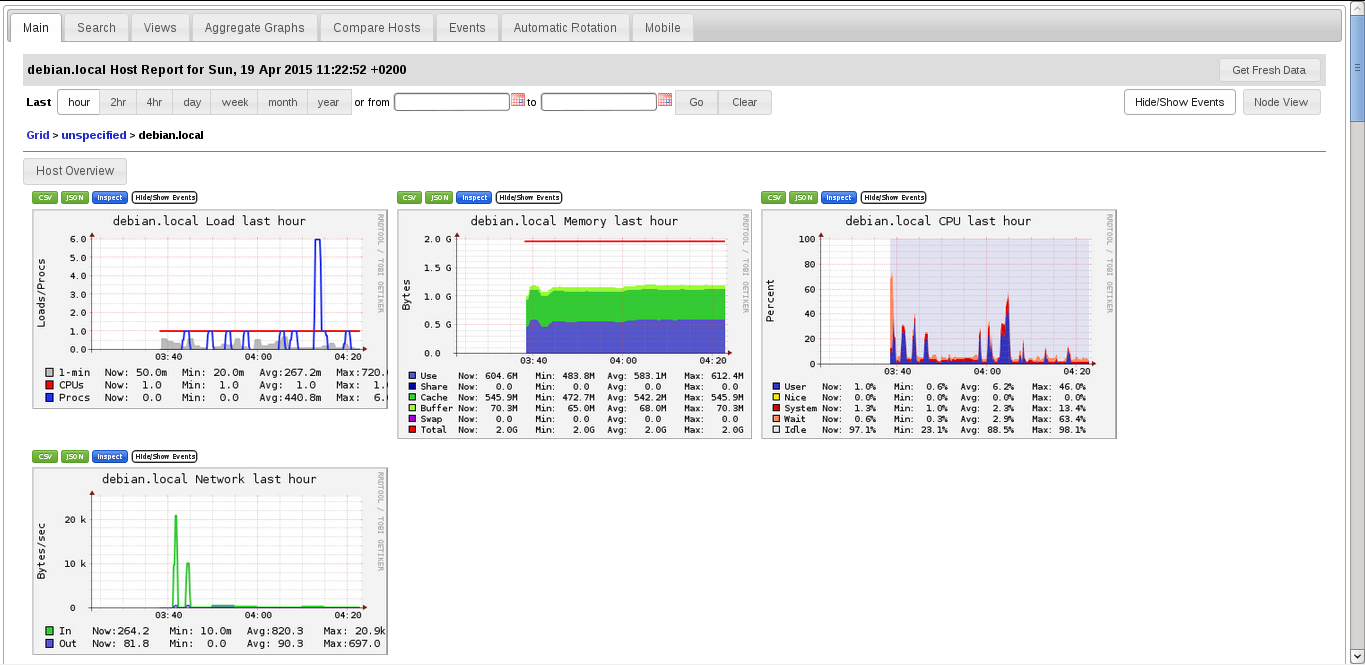
\includegraphics[scale=0.41]{ganglia.png}
	\end{center}
	\caption{Používateľské rozhranie nástroja Ganglia}
\end{figure}

\subsection{Výhody nástroja Ganglia}

Asi najväčšou výhodou nástroja Ganglia je to, že dokáže monitorovať celé clustre a gridy.
Je určená na agregáciu metrík z viacerých serverov a z komplexných informačných systémov.
To nám výrazne zjednoduší porovnávanie metrík získaných z viacerých inštalácií.

Na ukladanie metrík Ganglia používa RRD databázu, takže metriky nemusíme v Ganglii konfigurovať.
Výhodné je aj jednoduché prepojenie s nástrojom Naggios.

Ďalším plusom je možnosť použitia multicastu.
Ak náhodou niektorý monitorovaný uzol vypadne, gmetad si vyžiada údaje od ďalšieho gmond modulu.
Keďže každý gmond má informáciu o metrikách všetkých ostatných gmond modulov v tom istom clusteri,
metriky sa nestratia ale odošlú sa prostredníctvom iného gmond modulu. 
Dokonca pridanie nových uzlov do clustera je jednoduché a bez ďalšej konfigurácie.
% multicast

%\subsubsection{Nevýhody nástroja Ganglia}
\subsection{Nevýhody nástroja Ganglia}

V istom zmysle je nevýhodou Ganglie to, že nevie alertovať problémy v systéme.
To sa dá docieliť prepojením Ganglie s nástrojom Naggios.
Musíme teda integrovať do systému až dva nástroje.

Pôvodne sme si vybrali nástroj na ukladanie a zobrazovanie metrík pre systém AiS2 Gangliu.
Narazili sme však na problém, že v čase písania tejto práce ešte nebola Ganglia dostupná pre najnovší Red Hat.

% nevyuzitie pre dlhodobe,  redhat nevieme deploynut

%------------------------------------------------------------------------------------------------------------------------------

%\subsection{Graphite vs Zabbix vs Ganglia}
\section{Graphite vs Zabbix vs Ganglia}

Ako sme už písali, nástroj Graphite je vhodný na monitorovanie menších systémov.
Pre väčšie informačné systémy je lepšie použiť komplexnejší nástroj, ako napríklad Zabbix alebo Gangliu.
Tie nám ponúkajú viac užitočných funkcií, ktoré môžeme využiť.
Zabbix vie detekovať problémy a tie jednoduchšie aj vyriešiť (napríklad reštartom zlyhanej služby), 
	Ganglia zas dokáže monitorovať celé clustre a gridy a ponúka nám jednoduchú agregáciu grafov.
Záleží od komplexnosti systému, ktorý nástroj si vyberieme.

%%%%%%%%%%%%%%%%%%%%%%%%%%%%%%%%%%%%%%%%%%%%%%%%%%%%%%%%%%%%%%%%%%%%%%%%%%%%%%%%%%%%%%%%%%%%%%%%%%%%%%%%%%%%%%%%%%%%%%%%%%%%%%%

\chapter{Monitorovanie systému AiS2}

%------------------------------------------------------------------------------------------------------------------------------

%\subsection{Vlastná práca}
\section{Testovanie nástrojov}
% demo

Aby sme vedeli vyššie spomenuté nástroje porovnať a vybrať si vhodné nástroje na zbieranie a zobrazovanie metrík kvôli monitorovaniu systému AiS2, nástroje sme si najskôr vyskúšali.

Pre testovacie účeli sme si vytvorili jednoduchú webovú aplikáciu.
Keďže je systém AiS2 napísaný prevažne v programovacom jazyku java, za formu webovej aplikácie sme si zvolili JSP (Java Server Pages) stránky.
Vytvorené JSP stránky môžete vidieť v prílohách A - C.

Vo virtuálnom stroji sme si nainštalovali nástroj Statsd server, Graphite, Zabbix a Gangliu.
Po kliknutí na tlačidlo „Special Feature“ v prílohe A sa zavolá príslušná JSP stránka s názvom „sender“, ktorá má inštanciu Statsd klienta (príloha B), alebo integrovanú knižnicu Metrics (príloha C), ktoré odošlú metriku o stlačení tlačidla do príslušného nástroja na uloženie a zobrazenie metriky.

Týmto sme si spomínané nástroje vyskúšali aby sme ich vedeli detailnejšie porovnať.


%------------------------------------------------------------------------------------------------------------------------------

%\subsection{Monitorovanie systému AiS2 v reálnom čase}
\section{Monitorovanie systému AiS2 v reálnom čase}

Pre monitorovanie systému AiS2 v reálnom čase sme sa rozhodli použiť nástroj Metrics v kombinácii s nástrojom Ganglia.

Metrics sme si vybrali aj preto, lebo komunikácia medzi Statsd klientom a Statsd serverom po sieti môže spôsobyť zbytočné zaťaženie siete.
Metrics nepotrebuje oddeleného klienta od servera.
Ďalším dôvodom pre výber Metrics bol ten, že je to java knižnica a vzhľadom k tomu, že systém AiS2 je v jave, integrácia nástroja do systému nebola zložitá.
Keby AiS2 nebol v jave, najpravdepodobnejšie by sme sa rozhodli pre nástroj Statsd.

Gangliu sme si vybrali preto, že ponúka riešenie pre agregáciu metrík z viacerých inštalácií systému AiS2 na jedno miesto.
Metriky zo všetkých inštalácií potom môžeme zobraziť prehľadne v jednom grafe a porovnať jednotlivé inštalácie medzi sebou.

Gangliu sa nám však nepodarilo nasadiť na najnovšiu verziu Red Hat distribúcie, pretože Ganglia ešte nie je pre túto verziu dostupná.
Vybrali sme si teda nástroj Zabbix, ktorý má vďaka používaniu MySQL databázy potenciál okrem zbierania metrík v reálnom čase zbierať aj metriky dlhodobo za účelom hĺbkovej analýzy. 

Zabbix sme teda nasadili na testovacie, vývojové a ostré prostredie do akademického informačného systému AiS2.
Určili sme si, že budeme zbierať metriky ohľadom funkcionality systému - počet spustení dialógov a metriky ohľadom operačného systému a prehliadača používateľov systému, za časový interval 3 sekundy.
Po nasadení zberu metrík na ostrý server sme v špičke zaznamenali výrazné zaťaženie siete kvôli trojsekundovému intervalu odosielania metrík.
Rozhodli sme sa preto tento interval zmeniť na tridsať sekúnd.

Ešte skôr ako sa nám podarilo zbierať prvé metriky zo systému Ais2, 
	museli sme upraviť názvy metrík, ktoré produkoval nástroj Metrics a to tak, aby ich bol Zabbix schopný akceptovať.
Každú metriku však v Zabbixe trebalo najprv nakonfigurovať.

V konfigurácii metriky trebalo nastaviť jej meno, 
	jednoznačný kľúč vzhľadom na všetky metriky, 
	spôsob prijatia metriky (v našom prípade to bol Zabbix trapper čo je modul na prijatie metriky z iného nástroja) a jej typ (celé číslo, desatinné číslo, \ldots).

Konfigurácia v zabbixe bola pri 142 metrikách veľmi komplikovaná a náročná na čas.
Ak by sme potrebovali v budúcnosti pridať ďalšie metriky pre novú funkcionalitu, museli by sme dodatočne Zabbix konfigurovať.
To je dosť nevýhodné.
Ostatné nástroje, ktoré používajú RRD databázu sú tak oveľa flexibilnejšie a nepotrebujú konfiguráciu metrík.
Ak zaznamenajú novú metriku, jednoducho v strome metrík si vtvoria nový adresár podľa názvu a prefixu metriky.
Konfigurácia nových metrík je teda nulová.

Zabbix navyše nepodporuje jednoduché zlievanie metrík z viacerých inštalácií na jedno miesto s možnosťou porovnávania inštalácií.
Potvrdila sa nám teda naša hypotéza, že Zabbix nie je vhodný nástroj pre monitorovanie systému AiS2 v reálnom čase.

% momentalne chceme gangliu, tak sme testovali zabbix, ze bude zly, aktualne zabbix, metrics, vyuzitie aj dlhodobe 2 v 1? asi ani jedno..., zbieranie metrik
% ciel 18 instalacii porovnavat - Ganglia metrics, gmond gmetric, kniznica, 
% konfiguracia, grafy, ...
% zabbix experimenty datamining

%------------------------------------------------------------------------------------------------------------------------------

%\subsection{Dlhodobé monitorovanie systému AiS2}
\section{Monitorovanie systému AiS2 za účelom hĺbkovej analýzy}
%logstash, logy obe problemy nejdu jednym nastrojom...uz su logy, session, rrd, mysql

Monitorovanie systému AiS2 v reálnom čase nám dá dôležité informácie o tom, čo sa deje so systémom práve teraz.
Ak zbierame takéto dáta dostatočne dlho, vieme zistiť trendy, ako sa metriky menili v minulosti.
Zistíme tak, kedy sa systém najviac využíva, kedy najmenej a tomu môžeme prispôsobiť napríklad plánované odstávky systému.

Nás však zaujímajú aj komplexnejšie informácie o systéme a jeho používateľoch, ktoré sa jednoduchou metrikou pokryť nedajú.
Radi by sme zistili vzory používania jednotlivých dialógov v systéme AiS2, hlavne čo sa týka vhodnosti ich návrhu.
Potrebovali by sme identifikovať zle navrhnuté dialógy v systéme, aby sa dali sprehľadniť a zjednodušiť, aby neboli pre používateľov informačného systému metúce.

Táto informácia by sa dala získať monitorovaním používateľa v systéme a to tak, že by sme zaznamenávali spustené dialógy, čas na nich strávený a následne zatváranie týchto dialógov v rámci jednej session.
Ak by sa stalo, že používateľ by otvoril dialóg, o chvýľu by ho zavrel, pootváral by ďalšie, možno podobné dialógy, a nakoniec by sa vrátil k prvému, vyplnil by ho a odoslal, je pravdepodobné že správny dialóg hľadal, ale hneď ho nenašiel.
Ak sa tento scénar opakuje často u rôznych používateľoch systému, pravdepodobne nie je dialóg, či ľubovoľná iná informácia v systéme vhodne navrhnutá alebo je v systéme zle umiestnená.

Detekcia takýchto dialógov by výrazne prispela k zlepšeniu a skvalitneniu informačného systému.
Používatelia by sa tak v ňom vedeli lepšie orientovať a našli by hľadanú informáciu rýchlejšie.
Má pre nás preto detekcia takýchto dialógov zmysel.

Informácia z takéhoto monitorovania je už dosť komplexná.
Musí obsahovať minimálne informáciu o identifikátore aktuálnej session, čísla dialógu a čase medzi otvorením a zatvorením dialógu.
Tieto údaje už nevieme zakódovať do jednoduchej metriky.
Údaje spolu úzko súvisia, z toho dôvodu ich nemôžeme rozdeliť do viacerých metrík, 
	pretože by sme ich nevedeli interpretovať, analyzovať a porovnávať medzi sebou.
Na uloženie tejto informácie nevieme použiť RRD databázu.
Vhodnejšia je relačná databáza.

Mysleli sme si, že Zabbix bude vhodný nástroj na ukladanie takýchto štruktúrovaných dát, keďže metriky ukladá v relačnej databáze MySQL.
Neskôr sme si ale uvedomili, že síce Zabbix na ukladanie metrík používa relačnú databázu, ale takúto komplexnú metriku mu nevieme poslať z žiadného nástroja na zbieranie metrík, ktoré sme vyššie opisovali, keďže podporujú iba zbieranie jednoduchých metrík.


% TODO session, cloud, grid...

\newpage

%%%%%%%%%%%%%%%%%%%%%%%%%%%%%%%%%%%%%%%%%%%%%%%%%%%%%%%%%%%%%%%%%%%%%%%%%%%%%%%%%%%%%%%%%%%%%%%%%%%%%%%%%%%%%%%%%%%%%%%%%%%%%%%

\chapter*{Záver}
\addcontentsline{toc}{chapter}{Záver}

V tejto bakalárskej práci sme sa zaoberali monitorovaním informačných systémov, prečo je monitorovanie výhodné pre vývoj systému a ako nám môže pomôcť pri jeho rozvíjaní.

Popísali sme si tri prístupy k monitorovaniu a to monitorovanie informačného systému v reálnom čase, dlhodobé monitorovanie systému a monitorovanie systému za účelom hĺbkovej analýzy.

Navrhli sme algoritmus na monitorovanie informačných systémov od určenia cieľov monitorovania až po analýzu a vyvodenie dôsledkov monitorovania.

Porovnali sme open-source nástroje na zbieranie a vizualizáciu metrík, konkrétne sú to nástroje Statsd, Metrics, Graphite, Zabbix a Ganglia.
Povedali sme si o ich výhodách a nevýhodách vzhľadom na monitorovanie akademického informačného systému AiS2.
Vybrali sme si nástroje Metrics a Zabbix, a integrovali sme ich do systému AiS2.

Vytvorili sme jednoduchú webovú aplikáciu na demonštráciu nástrojov na zbieranie a zobrazovanie metrík.

Zistili sme, že by naše problémy ohľadom agregácie metrík z viacerých inštalácií a prehľadné porovnanie týchto inštalácií vyriešil omnoho lepšie nástroj Ganglia.
Takisto by nám to uľahčilo konfiguráciu oproti nástroju Zabbix



% otvorene problemy, ktore chceme riesit dalej 
%vyhody, nevyhody, aj napriek infrastruktury aj na aplikacne a pouzivatelske ale hlavne realtime pre rozsiahle cloudy Ganglia, ale naggios j riesenie komplexne nieje, nevyriesia ani jednu ulohu komplexne. Zabbix nie, lebo potencial databazy nevyvazi komplikovanu konfiguraciu, ani templates nepomozu. Dlhodobe relacna db je dobra, zabbix nie je plnohodnotny, metrics lepsi gmondy, metrics aj pise do logov, co bude pouzitelne pri dlhodobom monitorovani. Java, tak statsd, keby ne tak statsd...

%------------------------------------------------------------------------------------------------------------------------------

\bibliography{bakalarka}

\renewcommand{\bibname}{Zoznam použitej literatúry}
\begin{thebibliography}{42}
%\bibitem{1} Ipsum, L.: Lorem ipsum dolor sit amet.
	\bibitem{1} MATT MASSIE, Bernard Li. Monitoring with Ganglia. 1. ed. Sebastopol, CA: O'Reilly, 2013. ISBN 9781449329709.
	\bibitem{2} ALLSPAW, John a Jesse ROBBINS. Web operations. 1st ed. Sebastopol, CA: O'Reilly, c2010, xvii, 315 p. ISBN 1449377440.
\end{thebibliography}
%
\newpage

%%%%%%%%%%%%%%%%%%%%%%%%%%%%%%%%%%%%%%%%%%%%%%%%%%%%%%%%%%%%%%%%%%%%%%%%%%%%%%%%%%%%%%%%%%%%%%%%%%%%%%%%%%%%%%%%%%%%%%%%%%%%%%%

\chapter*{Prílohy}
\addcontentsline{toc}{chapter}{Prílohy}

\newcommand{\tab}[1]{\hspace{.05\textwidth}\rlap{#1}}

Príloha A: \tab{JSP stránka simulujúca webovú aplikáciu} \\
Príloha B: \tab{JSP stránka so Statsd klientom} \\
Príloha C: \tab{JSP stránka s integrovanou knižnicou Metrics} \\


% TODO zoznam priloh

\lstset{
	title=\lstname,
	basicstyle=\footnotesize,
	breaklines=true
}

\newpage

\section*{Príloha A}

\lstinputlisting{example.jsp}

\newpage

\section*{Príloha B}

\lstinputlisting{statsd_sender.jsp}

\newpage

\section*{Príloha C}

\lstinputlisting{metrics_sender.jsp}


\end{document}